
%---------------------------------------------------------------------
%	PAKKER
%---------------------------------------------------------------------

\documentclass[12pt,fleqn,a4paper]{report}
\usepackage[utf8]{inputenc}
\usepackage[danish]{babel}
\usepackage[top=2.5cm, left=2cm, right=2cm, bottom=2.5cm]{geometry}
\usepackage{graphicx}
\usepackage[bottom]{footmisc}
\usepackage{framed}
\usepackage{caption}
\usepackage{mdframed}
\usepackage{listings}
\usepackage{color}
\usepackage[T1]{fontenc}
\usepackage{amsmath,amsfonts,amsthm} % Math packages
\usepackage{array}
\usepackage{wrapfig}
\usepackage{multirow}
\usepackage{tabu}
\usepackage{underscore}
\usepackage{lastpage}
\usepackage{fancyhdr}
\usepackage[compact]{titlesec}
\usepackage[table,xcdraw]{xcolor}
\usepackage{arydshln}
\usepackage{mdframed}
\definecolor{mygreen}{RGB}{28,172,0} % color values Red, Green, Blue
\definecolor{mylilas}{RGB}{170,55,241}
\renewcommand{\lstlistingname}{Kodeudsnit}
\tabulinesep=3mm


\lstset{language=Matlab,%
    %basicstyle=\color{red},
    breaklines=true,%
    morekeywords={matlab2tikz},
    keywordstyle=\color{blue},%
    morekeywords=[2]{1}, keywordstyle=[2]{\color{black}},
    identifierstyle=\color{black},%
    stringstyle=\color{mylilas},
    commentstyle=\color{mygreen},%
    showstringspaces=false,%without this there will be a symbol in the places where there is a space
    emph=[1]{for,end,break},emphstyle=[1]\color{red}, %some words to emphasise
    %emph=[2]{word1,word2}, emphstyle=[2]{style},    
}


\makeatletter
\pagestyle{fancy}
\fancypagestyle{plain}{}
\fancyfoot{} % clear all fields
\fancyfoot[RO,RE]{Side \thepage\ af \pageref{LastPage}}
\fancyhead{} % clear all fields
\renewcommand{\headrulewidth}{0pt}

\def\thickhrulefill{\leavevmode \leaders \hrule height 1.2ex \hfill \kern \z@}
\def\@makechapterhead#1{
  \vspace*{10\p@}%
  {\parindent \z@ \centering \reset@font
        \thickhrulefill\quad 
        \scshape\bfseries\textit{\@chapapp{}  \thechapter}  
        \quad \thickhrulefill
        \par\nobreak
        \vspace*{10\p@}%
        \interlinepenalty\@M
        \hrule
        \vspace*{10\p@}%
        \Huge \bfseries #1 \par\nobreak
        \par
        \vspace*{10\p@}%
        \hrule
        \vskip 40\p@
  }}


\titlespacing{\subsection}{20pt}{*2}{*2}
\titlespacing{\subsubsection}{40pt}{*2}{*2}

\graphicspath{ {Figur/} }


%På figur~\ref{fig:fuld_lyd_tid}


%\begin{framed}
%\begin{center}
%	\includegraphics[width=\textwidth]{fuld_lyd_tid.png}
%	\captionof{figure}{Trafikstøj set i forhold til tiden} 
%	\label{fig:fuld_lyd_tid}
%\end{center}
%\end{framed}



%Se Kodeudsnit \ref{lstlisting:generel_kode}

%\captionof{lstlisting}{Generelle egenskaber for koden til fremstilling af diverse figure i matlab} 
%\label{lstlisting:generel_kode}
%\vspace{5mm} %5mm vertical space
%
%\subsection{Kode til lyd i forhold til tiden}
%\begin{framed}
%\begin{center}
%\begin{lstlisting}
%figure('name','trafikstoejen i fuld laengde'); clf
%subplot(211);
%plot(t,s_sound_left)
%xlabel('Tid (sek)')
%ylabel('Signalstyrke')
%title('Trafikstoej set i forhold til tiden')
%grid on
%hold on
%\end{lstlisting}
%\end{center}
%\end{framed}




\begin{document}
	
%---------------------------------------------------------------------
%	FORSIDE
%---------------------------------------------------------------------

\begingroup
\thispagestyle{empty}
\centering
\vspace*{5cm}
\par\normalfont\fontsize{35}{35}\sffamily\selectfont
\textbf{TCP socket fil overførsel}\\
{\LARGE IKN øvelse 7}\par
{\LARGE Gruppe 52}\par
\vspace*{1cm}
{\small
\begin{center}
\begin{tabu} to 1 \textwidth { X[l,1]  X[c,1] X[c,1] }
	Ragnar-Gwyn Dixen & 201400301 & au516263\\
	Thomas Sanberg Jensen & 201401914 & au513522\\
	Benjamin Kirkeby & 201410819 & au529001\\
	\end{tabu}
\end{center}}
\endgroup
\newpage


%---------------------------------------------------------------------
%	INDHOLD
%---------------------------------------------------------------------
\tableofcontents{}
\newpage

%---------------------------------------------------------------------
%	INDLEDNING
%---------------------------------------------------------------------
\chapter{Indledning}

\section{Opgaveformulering}
Denne journal skal beskrive udviklingsforløbet, funktionaliteten og resultatet for udviklingen af:
\begin{enumerate}
	\item En TCP-server med support for en client ad gangen, som kan modtage
	en tekststreng fra en client. Serveren skal køre i en virtuel Linux-maskine.
	Tekststrengen skal indeholde et filnavn, eventuel ledsaget af en stiangivelse.
	Tilsammen skal informationen i tekststrengen udpege en fil af en vilkårlig
	type/størrelse i serveren, som en tilsluttet client ønsker at hente fra serveren. Hvis filen ikke findes skal serveren returnere en fejlmelding til client’en. Hvis filen findes skal den overføres fra server til client i segmenter på 1000 bytes ad gangen – indtil filen er overført fuldstændigt. Serverens portnummer skal være 9000. Serverapplikationen skal kunne startes fra en terminal med kommandoen:
	\begin{lstlisting}[backgroundcolor = \color{lightgray}, language=bash]
	./file_server
	\end{lstlisting}
	Serveren skal være iterativ, dvs. den skal ikke lukke ned når den har sendt en fil til en client. Den skal, efter endt filoverførsel, kunne håndtere en ny forespørgsel fra en client (samme client eller en anden client).
	Serveren skal kun kunne håndtere en client ad gangen.
	
	\item Der skal udvikles en client kørende i en anden virtuel Linux-maskine. Denne client skal kunne hente en fil fra den ovenfor beskrevne server. Client’en sender indledningsvis en tekststreng, som er indtastet af operatøren, til serveren.
	Tekststrengen skal indeholde et filnavn + en eventuel stiangivelse til en fil i serveren. Client’en skal modtage den ønskede fil fejlfrit fra serveren – eller udskrive en fejlmelding hvis filen ikke findes i serveren. Client-applikationen skal kunne startes fra en terminal med kommandoen:
	\begin{lstlisting}[backgroundcolor = \color{lightgray}, language=bash]
	./file_server <file_servers ip-adr.> <[sti] + filnavn>
	\end{lstlisting}
	
	\item Som kvalitetskontrol for client/server systemet skal den overførte fil kunne sammenlignes med den oprindelige fil vha. terminal-kommandoen:
	\begin{lstlisting}[backgroundcolor = \color{lightgray}, language=bash]
	diff -s <afsendt fil> <modtaget fil>
	\end{lstlisting}
	<afsendt fil> er overført til client vha. af email, ftp eller anden pålidelig, ikke proprietær overføringsmetode.
	Der må ikke være forskel mellem filerne, hverken mht. til størrelse eller mht. indhold.

\end{enumerate}

%\section{Ordliste}
%\begin{center}
%	\begin{tabu} to 1 \textwidth { X[l,1.2]  X[l,4] }
%		\tabulinestyle{1pt}
%		\tabucline[1pt]{}
%		Ord & Forklaring  \\
%		\tabucline[2pt]{}
%		Aktivt valg  & Når brugeren skal foretage et valg med øjnene. Dette svare til et venstreklik med en almindelig mus \\
%		\tabucline[1pt on2pt]{}
%		Valgfelt  & Et felt på skærmen hvor brugeren skal foretage et aktivt valg \\
%		\tabucline[1pt on2pt]{}
%		Processindikator  & En indikation af hvor langt den operation, der er i gang, er kommet \\
%		\tabucline[1pt on2pt]{}
%		Dvaletilstand  & Systemet er lukket ned i en strømbesparende tilstand, men en modtager på robotten er aktiv, så denne vil kunne vågne til aktiv tilstand ved et signal fra PC applikationen \\
%		\tabucline[1pt on2pt]{}
%		Operationstilstand  & Når systemet er klar til at blive betjent af brugeren \\
%		\tabucline[1pt on2pt]{}
%		Robot  & Den styrbare enhed i systemet \\
%		\tabucline[1pt on2pt]{}
%		Udvidelsesmodul  & Et eksternt modul der kan sættes på robotten for at øge funktionaliteten. Dette vil kunne udvikles af tredjepartsudviklere  \\
%		\tabucline[1pt on2pt]{}
%		GUI  & En grafisk brugerflade med hvilken brugeren interagerer med systemet \\
%		\tabucline[1pt]{}	
%	\end{tabu}
%\end{center}


\newpage

%---------------------------------------------------------------------
%	SERVER
%---------------------------------------------------------------------
\chapter{TCP Server}


\section{Fremgangsmåde}
For at lave en TCP-server er der gjort brug af denne fremgangsmåde:
\begin{enumerate}
	\item Socket
	\item Bind
	\item Listen
	\item Accept
	\item Send
	\item Close
\end{enumerate}
De forskellige steps bliver beskrevet herunder.

\subsection{Socket}
\begin{framed}
\begin{lstlisting}[language=C++]
//Create socket
socket_desc = socket(AF_INET , SOCK_STREAM , 0);
if (socket_desc == -1)
{
	printf("Could not create socket");
}
\end{lstlisting}
\end{framed}
Her oprettes en socket. Det er denne socket, der bliver brugt og muliggøre forbindelsen mellem serveren og en klient. Hvis det ikke lykkes at oprette forbindelse, udskrives der en fejlmeddelelse i terminalen. 
\newpage
\subsection{Bind}
\begin{framed}
\begin{lstlisting}[ language=C++]
//Bind
if( bind(socket_desc,(struct sockaddr *)&server,
	sizeof(server)) < 0)
{
puts("bind failed");
return 1;
}
puts("bind done");
\end{lstlisting}
\end{framed}
Socket bliver bundet til serverens adresse. Dette muliggøre at en klient kan finde forbindelse ved hjælp af serverens ip adresse og portnummer. Der vil blive udskrevet en fejlmeddelelse i terminalen hvis dette ikke lykkes.

\subsection{Listen}
\begin{framed}
\begin{lstlisting}[language=C++]
//Listen
listen(socket_desc , 3);

puts("Waiting for incoming connections...");
\end{lstlisting}
\end{framed}
Listen funktionen gør, så serveren står og venter på at en klient vil forsøge at skabe en forbindelse. 

\subsection{Accept}
\begin{framed}
\begin{lstlisting}[language=C++]
//Accept an incoming connection
if((new_socket = accept(socket_desc, (struct sockaddr *)&client,(socklen_t*)&c))){
puts("Connection accepted");
}
\end{lstlisting}
\end{framed}
Når en klient har anmodet om en forbindelse, vil serveren validere på anmodningen. Hvis anmodningen er korrektvil den lave en accept. Derefter er der skabt forbindelse til klienten. 
\newpage
\subsection{Send}
\begin{framed}
\begin{lstlisting}[language=C++]
//Read message from socket (from client)
read(socket, read_buffer , 255);
\end{lstlisting}
\end{framed}
 Det første der bliver gjort i send_image() er at aflæse på forbindelsen ved hjælp af en read() funktion. Denne funktion aflæser hvilken sti og fil der bliver anmodet om fra klienten. 
 
\begin{framed}
\begin{lstlisting}[language=C++]
//Open file for future work
picture = fopen(read_buffer, "r");

//Verificationmessage to client (file exists)
write(socket, "1", sizeof(int));
\end{lstlisting}
\end{framed}
Der bliver derefter gjort brug af fopen() funktionen til at åbne stien og give den tilladelse til at aflæse.
Hvis denne sti og fil eksisterer, vil serveren sende en verifikations besked tilbage til klienten.

\begin{framed}
\begin{lstlisting}[language=C++]
//Picture size
printf("Getting Picture Size\n");
fseek(picture, 0, SEEK_END);
size = ftell(picture);
fseek(picture, 0, SEEK_SET);
printf("Total Picture size: %i\n",size);

//Send Picture Size
printf("Sending Picture Size\n");
write(socket, (void *)&size, sizeof(int));
\end{lstlisting}
\end{framed}
For at finde størrelsen på den fil som skal afsendes, er der brugt en fseek funktion. Denne funktion returnerer enten 0 eller en værdi som bliver returneret ved hjælp af ftell() funktionen. 
Størrelsen bliver derefter skrevet til klienten med en write() funktion.
\newpage
\begin{framed}
\begin{lstlisting}[language=C++]
while(!feof(picture)) {
//Read from the file into our send buffer
read_size = fread(send_buffer, 1, sizeof(send_buffer), picture);
	
//Send data through our socket
do{
stat = write(socket, send_buffer, read_size);
}while (stat < 0);
	
printf("Packet Number: %i\n",packet_index);
printf("Packet Size Sent: %i\n",read_size);
printf(" \n");
printf(" \n");
	
	
packet_index++;
	
//Zero out our send buffer
bzero(send_buffer, sizeof(send_buffer));
}
\end{lstlisting}
\end{framed}
De første 1000 bytes af filen bliver læst ind i en buffer ved hjælp af fread(). Denne buffer sendes til klienten ved hjælp af write(). Når bufferen er blevet sendt, tømmes den (fyldes med 0'er) ved hjælp af bzero(), for derefter at blive fyldt med de næste 1000 bytes indtil sidste bit i filen ved hjælp af feof().

 
\subsection{Close}
\begin{framed}
\begin{lstlisting}[language=C++]
//Close socket
close(socket_desc);
\end{lstlisting}
\end{framed}

Til sidst bliver socket forbindelsen lukket.
Dog skal kommunikationen være iterativ, dermed vil denne funktion ikke blive kørt, da koden fra "listen" til og med "send" er i et uendeligt loop.
\newpage

\chapter{TCP Klient}

\section{Fremgangsmåde}
For at lave en TCP-klient er der gjort brug af denne fremgangsmåde:
\begin{enumerate}
	\item Socket
	\item Connect
	\item Recieve
	\item Close
\end{enumerate}
De forskellige steps bliver beskrevet herunder.

\subsection{Socket}
\begin{framed}
	\begin{lstlisting}[language=C++]
//Create socket
socket_desc = socket(AF_INET , SOCK_STREAM , 0);
	\end{lstlisting}
\end{framed}

\subsection{Connect}
\begin{framed}
\begin{lstlisting}[language=C++]
//Socket setup
server.sin_addr.s_addr = inet_addr(argv[1]);
server.sin_family = AF_INET;
server.sin_port = htons( 9000 );
	
//Connect to remote server
if (connect(socket_desc , (struct sockaddr *)&server , sizeof(server)) < 0) {
cout<<strerror(errno);
close(socket_desc);
puts("Connect Error");
return 1;
}
	
puts("Connected\n");
\end{lstlisting}
\end{framed}

\subsection{Recieve}
\begin{framed}
\begin{lstlisting}[language=C++]
//Write file request to socket
stat = write(socket, file_direc, 512);
	
//Verification of file existence
char verification;
read(socket, &verification, sizeof(int));
	
if(verification == '0')
{
cout << "error finding the image!" << endl;
return 0;
}
	
cout << "succes finding the image!" << endl;
\end{lstlisting}
\end{framed}

\begin{framed}
\begin{lstlisting}[language=C++]
//Find the size of the image
do{
stat = read(socket, &size, sizeof(int));
}while(stat<0);
\end{lstlisting}
\end{framed}

\begin{framed}
\begin{lstlisting}[language=C++]
//Open corresponding file/filepath to store receiving image
image = fopen(file_direc, "w");
\end{lstlisting}
\end{framed}

\begin{framed}
\begin{lstlisting}[language=C++]
while(recv_size < size) {
	
	
FD_ZERO(&fds); //File descriptor set to zero
FD_SET(socket,&fds); //Add File descriptor set
	
// Indicates which of the specified file descriptors is ready for reading, writing, or has an error condition pending
buffer_fd = select(FD_SETSIZE,&fds,NULL,NULL,&timeout);
	
if (buffer_fd < 0)
printf("error: bad file descriptor set.\n");
	
if (buffer_fd == 0)
printf("error: buffer read timeout expired.\n");
	
if (buffer_fd > 0)
{
	// Reads the size of the recieved packet
	do{
		read_size = read(socket,imagearray, packet_size);
	}while(read_size <0);
	
printf("Packet number received: %i\n",packet_index);
printf("Packet size: %i\n",read_size);
	
	
//Write the currently read data into our image file
write_size = fwrite(imagearray,1,read_size, image);
printf("Written image size: %i\n",write_size);

if(read_size !=write_size) {
printf("error in read write\n");    }
	
	
//Increment the total number of bytes read
recv_size += read_size;
packet_index++;
printf("Total received image size: %i\n",recv_size);
printf(" \n");
printf(" \n");
}

}

fclose(image);
\end{lstlisting}
\end{framed}

\begin{framed}
	\begin{lstlisting}[language=C++]
	
	\end{lstlisting}
\end{framed}

\begin{framed}
	\begin{lstlisting}[language=C++]
	
	\end{lstlisting}
\end{framed}

\begin{framed}
	\begin{lstlisting}[language=C++]
	
	\end{lstlisting}
\end{framed}


\subsection{Close}
\begin{framed}
\begin{lstlisting}[language=C++]
// closes the socket connection
close(socket_desc);
\end{lstlisting}
\end{framed}

\newpage

På figur~\ref{fig:dele_i_system} ses en illustration af de forskellige dele systemet består af. Der er vist, at brugeren kigger på GUI’et, imens kameraet skanner brugerens øje. PC’en kommunikere trådløst med bilen, der har påmonteret et kamera.

\begin{center}
	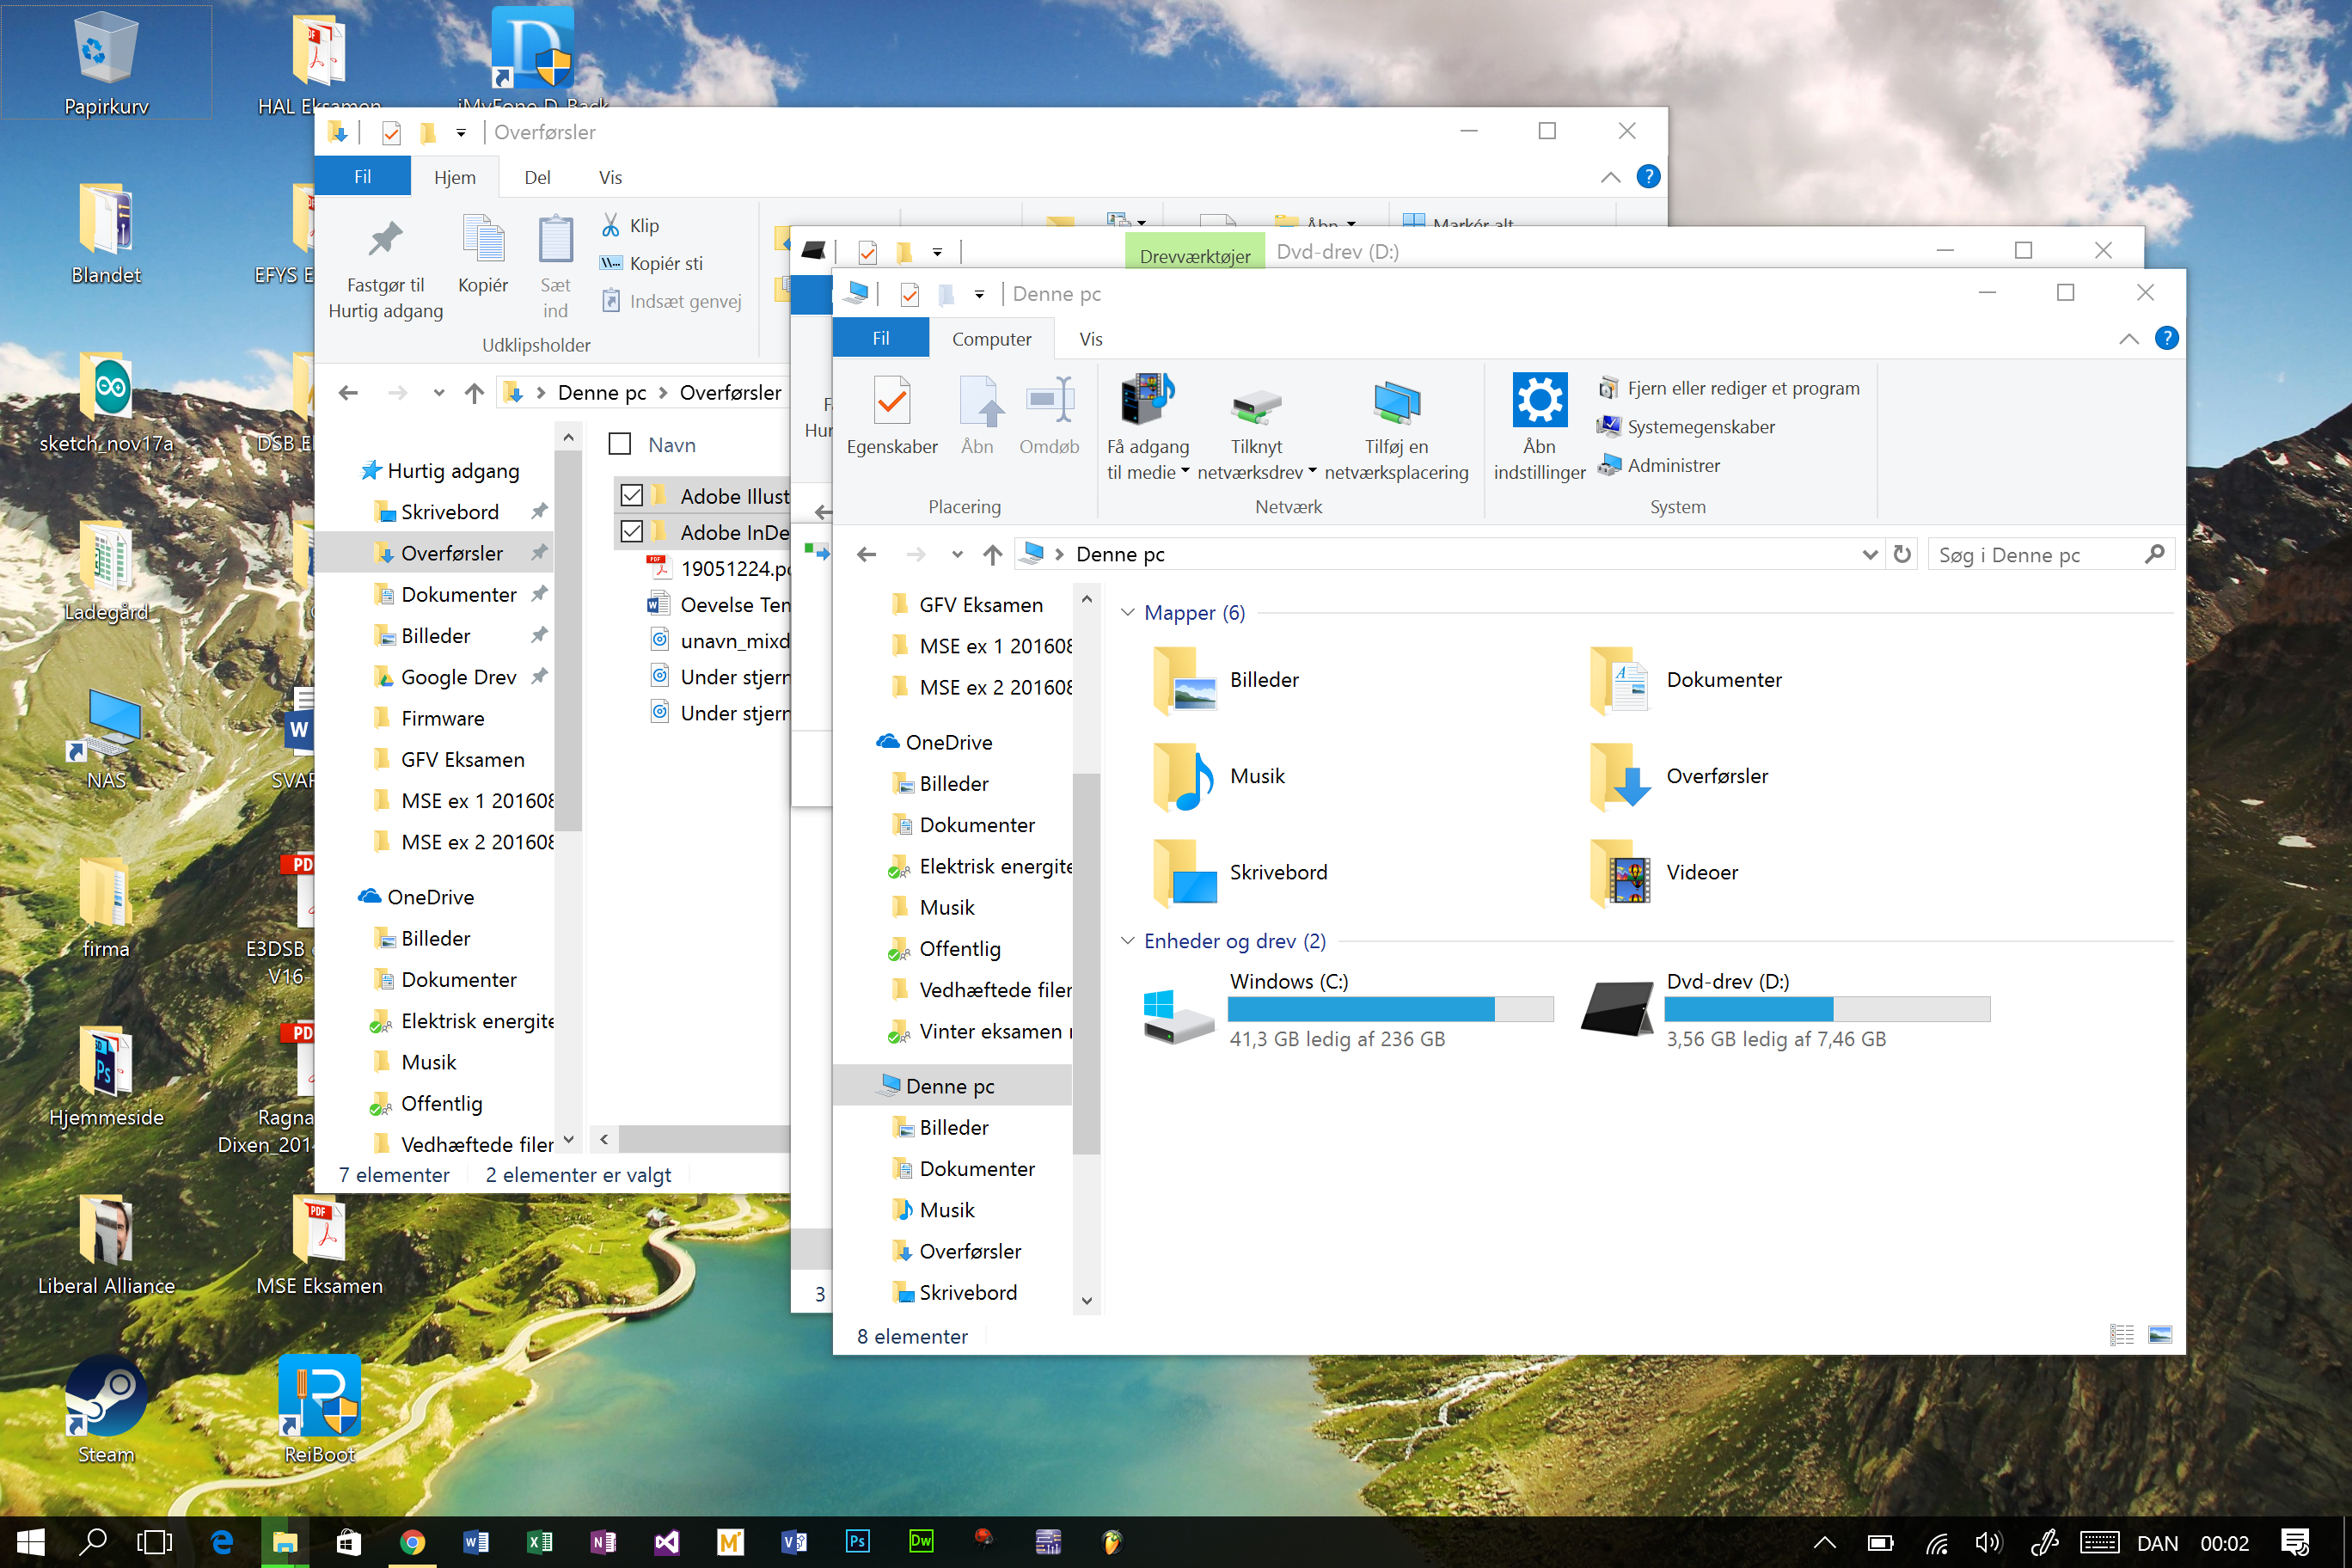
\includegraphics[width=0.9 \textwidth]{hej1.png}
	\captionof{figure}{Illustration af de forskellige dele systemet består af}
	\label{fig:dele_i_system}
\end{center}

\newpage



\end{document}